% !TEX root = knauss-vissuelizer.tex
\section{V:Issue:lizer}


\viss\  is an interactive tool that allows software developers and managers to dynamically explore the discussion of requirements  in online repositories with a focus on highlighting the difference between clarification and implementation related communication. (Source code available at \url{https: //github.com/oerich/ReqtDisc})


The main window shows a list of requirements on the  left \todo{\footnotesize move to conclusion: (e.g. workitems in jazz, items in jira, issues in other systems)} (see Figure \ref{fig:screenshot}).
\viss\ adds visualizations to the selected discussions in the centre or in an extra window. 
These visualizations help to assess the communication through discussion events (e.g. comments) that are related to these requirements.
The panel on the right allows users to adjust parameters of the visualization.
Most importantly, the resolution of time intervals for the visualization can be adjusted, either as a fixed number of intervals (e.g. eight intervals in Figure \ref{fig:example-trajectory}), or as a fixed time interval (e.g. days, weeks, month).
%
\viss\  offers  two visualizations: 

\subsubsection{Clarification Trajectories} 
This visualization shows how the percentage of clarification events to other discussion events related to a requirement changes over its lifetime.
\begin{figure}[b]
\centering
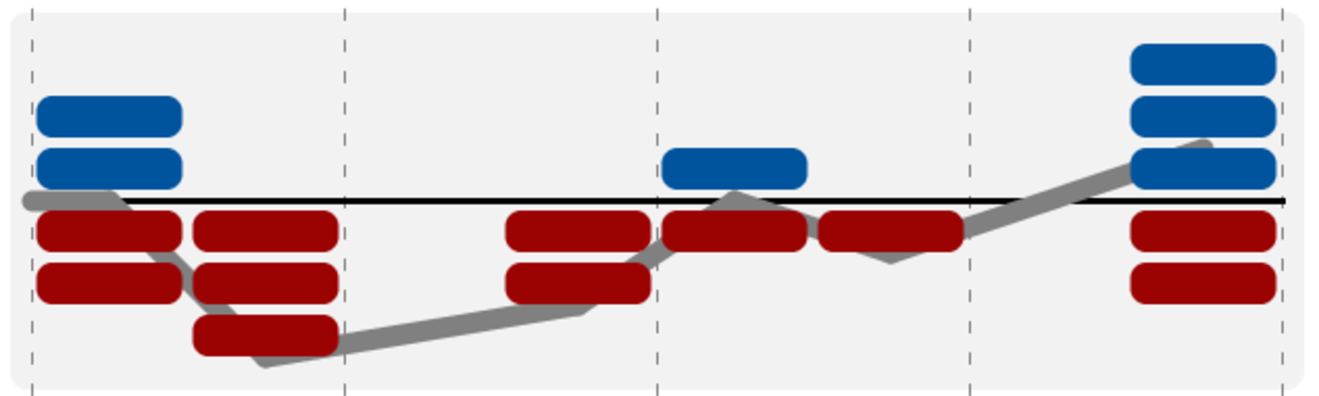
\includegraphics[width=0.51\columnwidth]{img/example-trajectory}
\caption{Example of a requirements discussion's clarification trajectory}
\label{fig:example-trajectory}
\end{figure}
Since the visualization of the clarification trajectory (see Figure \ref{fig:example-trajectory}) is a new concept, it needs some explanation.
The black line represents the lifetime of the requirement discussion from the creation of the requirement in the system to the last recorded discussion event.
Dashed lines divide the lifeline into quarters and help to locate in which part of the lifetime discussion occurs.
Discussion events are depicted by rectangles that are shown below the lifeline if they are clarification events, and above the lifeline if they are not.
A grey line shows the sum of clarification.
In a classic trajectory with clarification up-front and only implementation related communication in the end, this grey line will start in the bottom left corner and raise to the upper right corner.
% For increased readability, the different types of discussion events are coloured in the tool (clarification events: red, other: blue).
\viss\ currently uses a Bayesian classifier to identify clarification events, i.e. a supervised machine learning algorithm.
Based on this classification, \viss\ generates trajectories and identifies reoccurring patterns (\emph{textbook-example, indifferent, discordant, procrastination, back-to-draft, and happy-ending}) \cite{Knauss2012f}.
Typically, there are many requirements without pathological findings, e.g. user stories with some clarification in the beginning and other communication events later on that show progress.
More suspicious trajectories show large amounts of clarification late in the iteration, perhaps even after the issue seemed to be solved. Others show no clarification at all, even though the requirement seems to be complex.
\subsubsection{Social Networks} 
This visualization shows the communication pattern of those participating in a requirement's discussion. 
The developers are presented as nodes and connections between nodes are weighted by the amount of communication both developers share about the requirement in a specific time interval (as defined above) in a requirement's lifetime. 
Thus, subgraphs of the contributors to the discussion in each time interval are created.
Two subgraphs are connected if  stakeholders appear in several time intervals. 
%Note that subgraphs can be matched to specific time intervals (here: three) where all actors of the subgraph communicate. 
%The interval can be a either a either a fixed number (here: three intervals), or a fixed time interval (e.g. days, weeks, month). 
\viss\ also displays the developer node as a pie chart to show the percentage of clarification vs. implementation-related communication in which the developer is involved (as highlighted in Figure \ref{fig:example-sn-large}).




% integrates information of the automatic analysis of online communication into the social networks, i.e. showing a pie chart with the percentage of clarification and implementation related communication for this developer.

